\documentclass[12pt]{article}
\usepackage[english]{babel}
\usepackage{natbib}
\usepackage{url}
\usepackage[utf8x]{inputenc}
\usepackage{amsmath}
\usepackage{graphicx}
\usepackage{subcaption}
\graphicspath{{images/}}
\usepackage{parskip}
\usepackage{fancyhdr}
\usepackage{vmargin}
\usepackage[shortlabels]{enumitem}


\setmarginsrb{3 cm}{2.5 cm}{3 cm}{2.5 cm}{1 cm}{1.5 cm}{1 cm}{1.5 cm}

\title{Ultrasound Quality Assurance}					% Title
\author{U.G.C. Jayasankha}								% Author
\date{\today}											% Date
\def \topic{Diagnostic Ultrasound}

\makeatletter
\let\thetitle\@title
\let\theauthor\@author
\let\thedate\@date
\makeatother

\pagestyle{fancy}
\fancyhf{}
\rhead{\theauthor}
\lhead{\thetitle}
%\chead{170259P}
\cfoot{\thepage}

\begin{document}

%%%%%%%%%%%%%%%%%%%%%%%%%%%%%%%%%%%%%%%%%%%%%%%%%%%%%%%%%%%%%%%%%%%%%%%%%%%%%%%%%%%%%%%%%

\begin{titlepage}
	\centering
    \vspace*{0.5 cm}
    
\includegraphics[scale = 0.8]{University_of_Moratuwa_logo.png}\\[1.0 cm]	% University Logo
    \textsc{\Large Department of Electronics and Telecommunication Engineering}\\[0.8 cm]
    %\textsc{\Large University of Moratuwa}\\[1.0 cm]	% University Name
	\textsc{\large BM 3121}\\[0.5 cm]				% Course Code
	\textsc{\Large Medical Imaging}\\[0.5 cm]				% Course Name
	\rule{\linewidth}{0.2 mm} \\[0.4 cm]
	{ \huge \bfseries \thetitle}\\
	\rule{\linewidth}{0.2 mm} \\[1.5 cm]
	
	\begin{minipage}{0.4\textwidth}
		\begin{flushleft} \large
			\emph{Name:}\\
			\theauthor
			\end{flushleft}
			\end{minipage}~
			\begin{minipage}{0.4\textwidth}
			\begin{flushright} \large
			\emph{Index Number:} \\
			170259P									% Your Student Number
		\end{flushright}
	\end{minipage}\\[2 cm]
	
	{\large \thedate}\\[2 cm]
 
	\vfill
	
\end{titlepage}

%%%%%%%%%%%%%%%%%%%%%%%%%%%%%%%%%%%%%%%%%%%%%%%%%%%%%%%%%%%%%%%%%%%%%%%%%%%%%%%%%%%%%%%%%

\tableofcontents
\pagebreak

%%%%%%%%%%%%%%%%%%%%%%%%%%%%%%%%%%%%%%%%%%%%%%%%%%%%%%%%%%%%%%%%%%%%%%%%%%%%%%%%%%%%%%%%%

\section{Introduction to \topic}
\subsection{Basics of \topic}
Medical Ultrasound or Diagnostic-Sonography is a medical procedure of using high frequency sound waves to image inside of the body. Ultrasound imaging was invented in 1956. It can be used to display dynamic visual images in most parts of the body such as  tendons, muscles, joints, blood vessels, and internal organs. Ultrasound imaging is the most popular imaging modality after projection x-ray imaging. Ultrasound imaging is predominantly used to image and diagnose pregnant mothers, which is known as "obstetric ultrasound" since ultrasound does not use ionizing radiations for imaging, thus no harm to the fetus. Ultrasound is also highly used to image soft tissues such as breast, tendons, thyroid, parathyroid glands and testes.

\begin{figure}[h!]
  \centering
  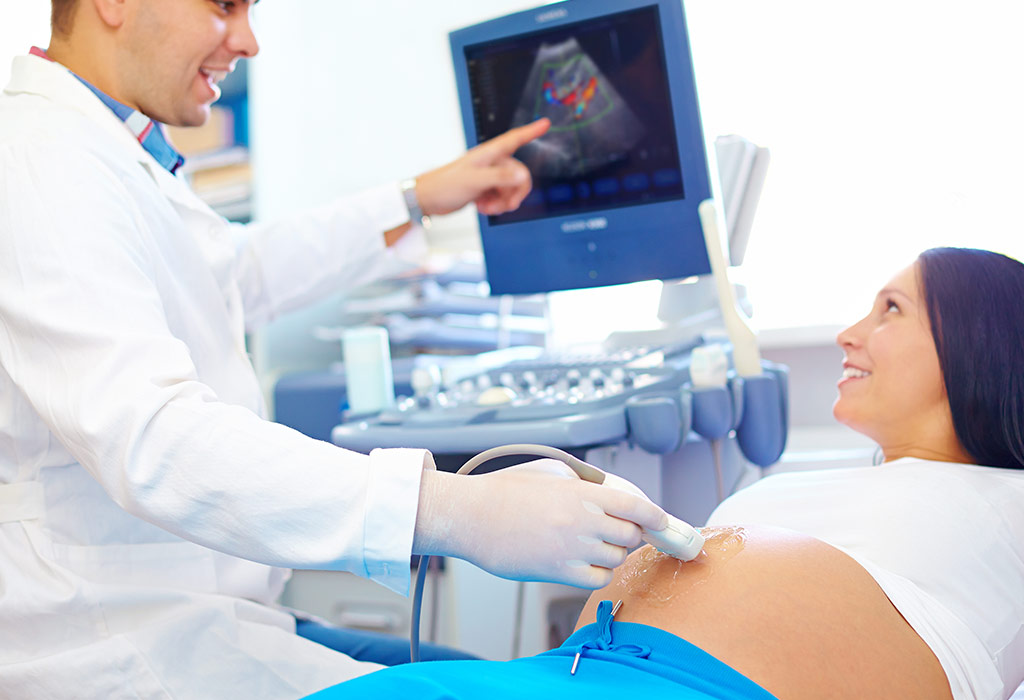
\includegraphics[width=0.8\linewidth]{U2.jpg}
  \caption{\small{Ultrasound Imaging of a pregnant woman}}
  \label{fig:Ultrasound Imaging}
\end{figure}

Physics of the ultrasound imaging is the echoing nature of sound waves. When the sound waves travel through a medium it attenuates. When the sound waves hit a boundary part of the wave transmits to the second medium and other part reflects back to the first medium. When this reflecting wave is detected it is proof for existing boundary. And using the time difference the distance to the boundary can be calculated if the speed of sound wave is known. Several reflection wave fronts will arrive at the receiver if there are several boundaries. 

There are 4 modes in ultrasound imaging. 
\begin{enumerate}[i.]
    \item \textbf{A-mode / Amplitude mode} -  the simplest type of ultrasound. A single transducer scans a line through the body with the echoes plotted on screen as a function of depth. 
    \item \textbf{B-mode / Brightness mode} - is the display of 2D map of B-Mode data, and is the most common form of ultrasound imaging. Unlike A-Mode, B-Mode is based on brightness with the absence of vertical spikes. The brightness depends upon the amplitude or intensity of the echo.
    \item \textbf{M-mode / Motion mode} - a rapid sequence of B-mode scans whose images follow each other in sequence on screen enables doctors to see and measure range of motion, as the organ boundaries that produce reflections move relative to the probe.
    \item \textbf{Doppler mode} - This mode makes use of the Doppler effect in measuring and visualizing blood flow. Doppler sonography play important role in medicine. Sonography can be enhanced with Doppler measurements, which employ the Doppler effect to assess whether structures (usually blood) are moving towards or away from the probe, and its relative velocity. 
\end{enumerate}

\begin{figure}[h!]
  \centering
  \begin{subfigure}[b]{0.32\linewidth}
    \centering
    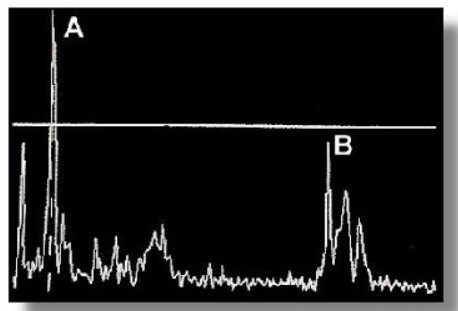
\includegraphics[width=1\linewidth]{A.jpg}
    \caption{A-mode}
  \end{subfigure}
  \begin{subfigure}[b]{0.32\linewidth}
    \centering
    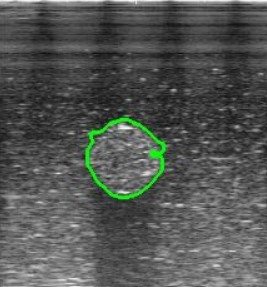
\includegraphics[width=1\linewidth]{b.jpg}
    \caption{B-mode}
  \end{subfigure}
  \begin{subfigure}[b]{0.32\linewidth}
    \centering
    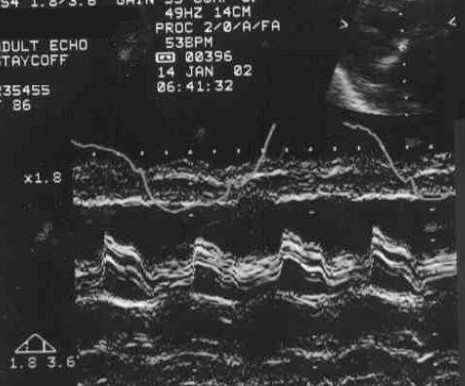
\includegraphics[width=1\linewidth]{m.jpg}
    \caption{M-mode}
  \end{subfigure}
  \caption{Modes of Ultrasound}
  \label{fig:Projectional Radiography}
\end{figure}

\pagebreak
\subsection{Importance of \topic}
Ultrasound scanning is ranked second after x-ray imaging as most used imaging modality. There are several reasons for that.   
\begin{enumerate}
    \item Ionizing radiation is not used\newline
    X-ray, CT, PET modalities of imaging use ionizing radiation which is harmful for the organs. But in Ultrasound imaging; ionizing radiation is not used. Therefore it is not harmful for the organs. 
    % \newline
    \item Inexpensive equipment \& low cost scans \newline
    When compared with other imaging modalities, Ultrasound scanners are less complicated. Therefore the system is inexpensive and maintenance cost is low. People can afford Ultrasound imaging modality easily.  
    
    \item High temporal resolution\newline
    Ultrasound can be operated in higher frame rates. Thus images can be acquired in short periods of time. Movements of organs such as moving baby,beating heart can be seen because of high frame rate. 
  
   % \newline
    \item Flow velocity measurement availability\newline
    Using Doppler effect, velocity of moving fluids in the body can be calculated. This can be useful to identify flow direction.Fluid moving patterns can be modeled.  
    
    \item Portability\newline
    Ultrasound scanner are light and smaller when compared with other modalities. It does not need an dedicated imaging room. It can be used in any ward and can be transported somewhere else easily. 
    
\end{enumerate}
But there are several disadvantages also. 
\begin{enumerate}
    \item Ultrasound imaging is not usable in bony or airy regions of body. Ex: Lungs  
    \item Field of view is limited. Can not get clear, accurate images as MRI or X-ray
    \item Quality of imaging depends on the operator.  
    \item Ultrasound images are hard to interpret. Experience is a must to interpret ultrasound images.
    \item Artefacts are common.
\end{enumerate}
\pagebreak

\subsection{Components and Implementation of \topic}

\begin{figure}[h!]
    \centering
    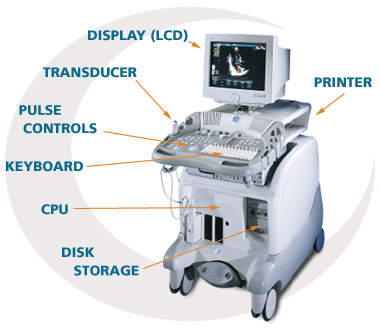
\includegraphics[width=0.6\linewidth]{us.png}
    \caption{\small{Main components of \topic}}
    \label{fig:Main components of US}
\end{figure}
All the main components of US system are shown in above figure. After applying gel on the imaging area of the body, using the transducer imaging is done. This is less complicated than other modalities. 

\begin{figure}[h!]
    \centering
    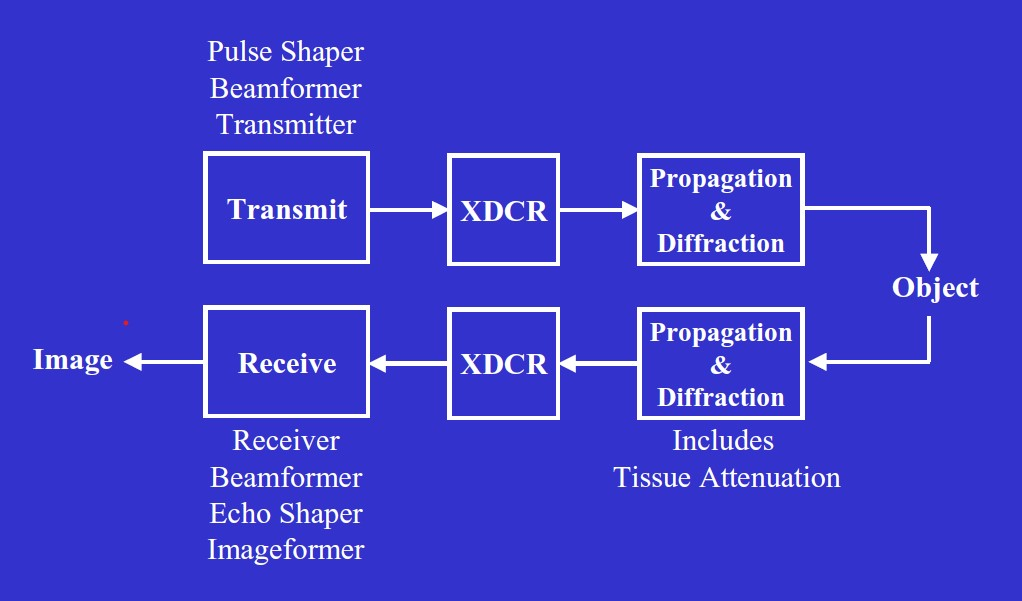
\includegraphics[width=0.75\linewidth]{u3.jpg}
    \caption{\small{Imaging system block diagram}}
    \label{fig:Imaging system block diagram}
\end{figure}
% Components of the \topic ,
% \begin{enumerate}
%     \item Powerful superconductor magnet - 1.5T / 3T / 6T
%     \item Gradient coils
%     \item Radio Frequency coils
%     \item Patient table
%     \item Shield
%     \item Computer system
    
% \end{enumerate}

\pagebreak
\section{Quality Assurance of \topic}
Ultrasound is a widely used imaging modality when compared with other imaging modalities since they are cheaper and harmless. However quality assurance of Diagnostic ultrasound is not a popular topic as quality assurance of other imaging modalities. Other imaging modalities are very complex and expensive equipment. Thus quality assurance methods are followed strictly. But due to some reasons people tend to neglect quality assurance methods of ultrasound. Here are the reasons for that given by people who refuses QA measures,

\begin{enumerate}[i.]
    \item Ultrasound is considered as a safe imaging modality. Thus QA measures are not needed
    \item Ultrasound Imaging systems are stable. Therefore QA measures are not necessary. 
    \item There are no dedicated operator or engineer for Ultrasound systems. Even the systems are being moved to different sections. Thus nobody knows how, what and when to test.
    \item No well established rules and regulations. 
\end{enumerate}

\begin{figure}[h!]
    \centering
    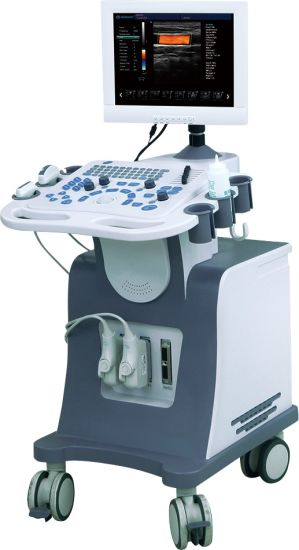
\includegraphics[width=0.35\linewidth]{u4.jpg}
    \caption{\small{Movable Ultrasound scanners}}
    \label{fig:Movable Ultrasound scanners}
\end{figure}

But these reasons are not accurate. Even though ultrasound scanners were used more than 50 years as a safe modality it had been revolutionary developed through past few years. In the beginning it was a simple system but now it is a compact system with various components. Due to competitive nature between vendors of ultrasound systems they try to overcome other using new technologies. Therefore most of the new ultrasound scanners use high power output. Even though it is not proved, there are evidence that high power outputs can harm the subject. Therefor quality assurance methods and rules and regulations are needed to limit exposure time, minimize scan times, reduce repeat rates and assure that scan protocols employ proper scanner settings. Even though Ultrasound systems are stable than other modalities, faults can occur gradually. A quality assurance measures can identify these faults or damages at the beginning. So it can be repaired with a low cost. 

Not every Ultrasound scanner is not expected to exhibit failures but ultrasound equipment is not immune to failures. Therefore Quality assurance measures are are expected to be followed. Otherwise failures may go unnoticed and cause sever damages to the system and diagnosis may be wrong. 

As in the other imaging modalities \textbf{phantoms} are used for quality assurance tests of \topic . 

Following are the \textbf{Quality assurance test and methods} for \topic
\begin{enumerate}
    \item System Sensitivity test
    \begin{enumerate}[a.]
        \item Maximum Depth of Penetration
        \item Speckles, artefacts and Noise
    \end{enumerate}
    \item Spatial Accuracy test
    \begin{enumerate}[a.]
        \item Volume Measurement
        \item Horizontal and vertical Distance Accuracy
    \end{enumerate}
    \item Uniformity test
    \begin{enumerate}[a.]
        \item Horizontal Uniformity
        \item Vertical Uniformity
    \end{enumerate}
    \item Contrast Resolution test
    \begin{enumerate}[a.]
        \item High Contrast Detctability test
        \item Low Contrast Object Detctability test
    \end{enumerate}
    \item Spatial resolution test
    \begin{enumerate}[a.]
        \item Horizontal resolution
        \item Vertical Resolution
    \end{enumerate}
\end{enumerate}

\section{Phantoms for Diagnostic Ultrasound QA}
Phantoms are used for quality assurance purposes to measure relevant parameters. These phantoms are specially designed for Ultrasound to represent the human body and mimic the human nature. Following imporatant features should be similar in phantom and the human body. 
\begin{enumerate}[i.]
    \item Attenuation Coefficient 
    \item Speed of Sound
    \item Back-scatter Coeffucient
    \item Mechanical Properties
    \item Thermal Properties
    \item Elasticity
\end{enumerate}
\subsection{TMM based Phantoms}
There are special substances which have above features similar to human tissues. Those substances are known as Tissue Mimicking Materials(TMM). They are used to manufacture Ultrasound phantoms. 
\begin{enumerate}[i.]
    \item Urethane
    \item Agar
    \item Zerdine
    \item TPE
\end{enumerate}
These are solid non-water based materials. Advantages of these TMM are,
\begin{itemize}
    \item Not subject to desiccation
    \item No need for scanning window
    \item Produce tissue-like backscatter
\end{itemize}
Disadvantages are,
\begin{itemize}
    \item Velocity is lower than tissue
    \item Attenuation is not proportional to frequency.
    \item Surface easily gets damaged if not cleaned
\end{itemize}

\begin{figure}[h!]
    \centering
    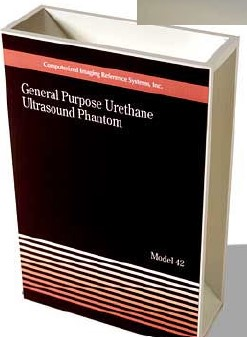
\includegraphics[width=0.35\linewidth]{tmm.jpg}
    \caption{\small{TMM based phantom}}
    \label{fig:TMM based phantom}
\end{figure}

\subsection{Water based phantoms}
Water based phantoms have some advantages over TMM based phantoms,
\begin{itemize}
    \item Velocity is similar to tissue
    \item Attenuation is proportional to frequency.
    \item Back-scattering property
\end{itemize}
\begin{figure}[h!]
    \centering
    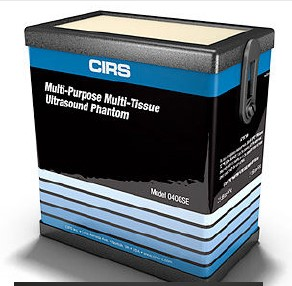
\includegraphics[width=0.45\linewidth]{water.jpg}
    \caption{\small{Water based phantom}}
    \label{fig:Water based phantom}
\end{figure}

But there are few disadvantages also,
\begin{itemize}
    \item Subject to desiccation
    \item Should be kept in containers
    \item Scanning window is required
\end{itemize}


\newpage
\pagebreak
\section{Main Quality Assurance Methods of \topic}
This section describes the main quality assurance methods used in diagnostic ultrasound. 

\subsection{Visual Checklist}
This is the basic method to find flaws in the system and it should be done in every week. Following list of equipment is inspected visually to find any missing part or any malfunction. This verifies whether the US system working properly electrically and mechanically. 

Visual checklist is divided into three sections

\subsubsection{Infection control and scanner damage}
\begin{figure}[!h]
    \centering
    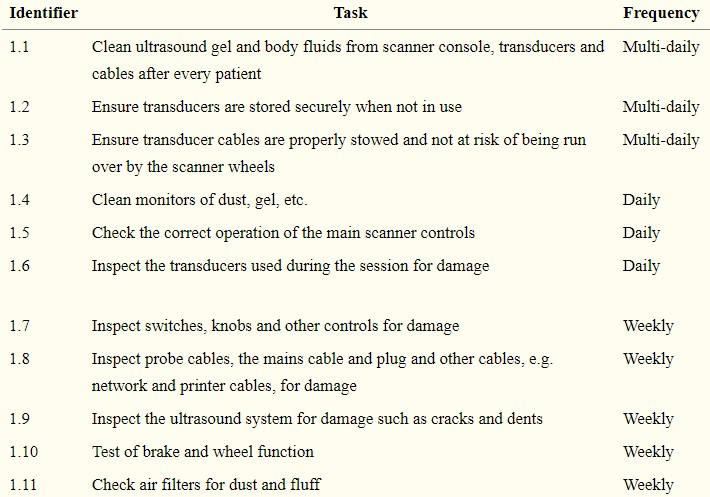
\includegraphics[width=0.8\linewidth]{vc.jpg}
    \caption{\small{Visual checklist step 1}}
    \label{fig:Visual checklist for US}
\end{figure}

\subsubsection{Basic scanner and transducer testing}
\begin{figure}[!h]
    \centering
    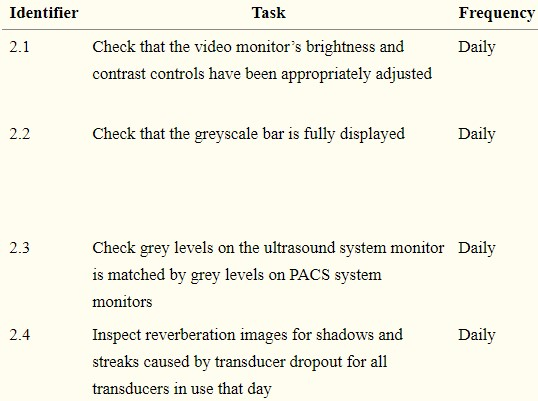
\includegraphics[width=0.8\linewidth]{vc1.jpg}
    \caption{\small{Visual checklist step 2}}
    \label{fig:Visual checklist for US}
\end{figure}

\subsubsection{Further scanner and transducer testing}
\begin{figure}[!h]
    \centering
    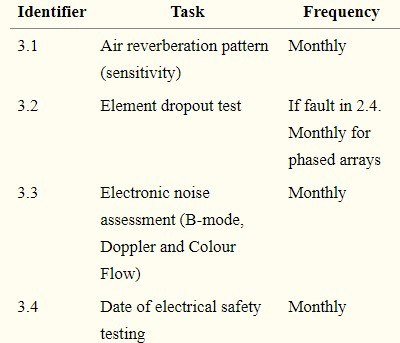
\includegraphics[width=0.6\linewidth]{vc2.jpg}
    \caption{\small{Visual checklist step 3}}
    \label{fig:Visual checklist for US}
\end{figure}


If any of this fails, it should be repaired or replaced as soon as possible even before carrying out other quality assurance protocols. 

\subsection{System Sensitivity test}
\subsubsection{Maximum Depth of Penetration/Visualization}
Maximum visual depth or maximum penetration depth is the maximum depth which can be seen through image. This is a axial measure of sensitivity. It is considered by as a overall check of the integrity of the US system. 
\begin{figure}[!h]
    \centering
    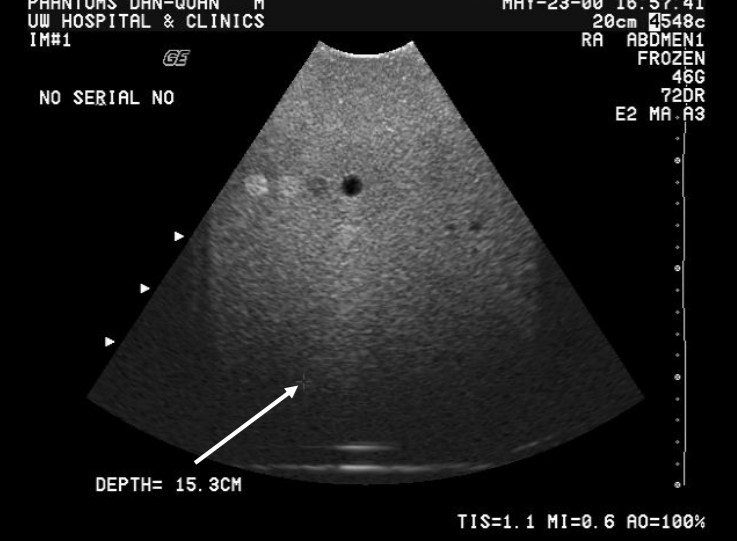
\includegraphics[width=0.6\linewidth]{md.jpg}
    \caption{\small{Maximum Depth of Penetration}}
    \label{fig:Maximum Depth of Penetration}
\end{figure}
\subsubsection{Speckles, artefacts and Noise}
\textbf{Speckles} - Abnormalities arose from the destructive and constructive nature of sound waves. This is due to the reflection of sound waves hitting small bodies. 
\begin{figure}[!h]
    \centering
    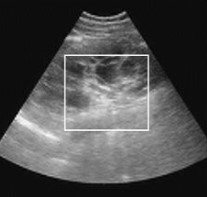
\includegraphics[width=0.25\linewidth]{speckle.jpg}
    \caption{\small{Speckles in \topic}}
    \label{fig:Speckles in US}
\end{figure}

\textbf{Artefacts} - Abnormalities that does not have any relation with the actual bodies/structures. Speckles are also artefacts in general. 
\begin{figure}[!h]
    \centering
    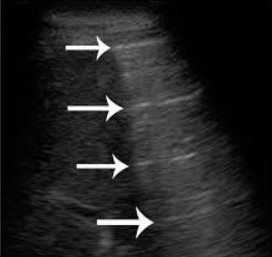
\includegraphics[width=0.25\linewidth]{ar.jpg}
    \caption{\small{Artifacts in \topic}}
    \label{fig:Speckles in US}
\end{figure}
\textbf{Noise} - Noise is the unwanted additional parts of the signal/image. Imperfections of the transducer or any other part of the system can generate noises. To achieve a great quality image, this noise part should be suppressed. \textbf{SNR Measurement} is the parameter to identify the noise level. SNR ratio decreases with the depth increases. 
\begin{figure}[!h]
    \centering
    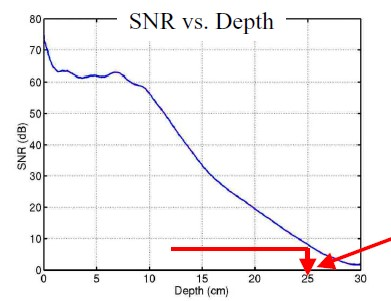
\includegraphics[width=0.3\linewidth]{snr.jpg}
    \caption{\small{SNR vs Depth}}
    \label{fig:SNR vs Depth}
\end{figure}


\subsection{Uniformity test}
Uniformity test is considered as the most important and useful test. In an ideal image,
\begin{itemize}
    \item No evidence of elements dropout
    \item No vertical shadows
    \item No loss of sensitivity near edges
\end{itemize}
\subsubsection{Horizontal Uniformity}
Horizontal non-uniformity is caused by malfunctioning transducer unit/element in the array. This can be identified by using a phantom. Following figure shows a such situation. 
\begin{figure}[!h]
    \centering
    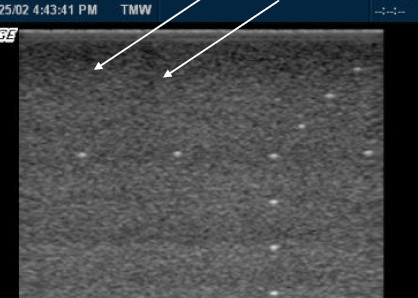
\includegraphics[width=0.6\linewidth]{un.jpg}
    \caption{\small{Horizontal Uniformity defects}}
    \label{fig:Horizontal Uniformity defects}
\end{figure}
\subsubsection{Vertical Uniformity}
Vertical non-uniformity occurs due to the attenuation of the sound waves. However, Time Gain Compensation (TGC) is used to produce a vertically uniform output. When Time Gain Compensation has any fault vertical non-uniformity can occur. 
\begin{figure}[!h]
    \centering
    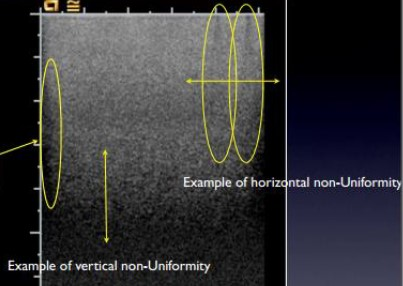
\includegraphics[width=0.6\linewidth]{vu.jpg}
    \caption{\small{Vertical Uniformity defects}}
    \label{fig:Vertical Uniformity defects}
\end{figure}

\subsection{Spatial Accuracy test}
\subsubsection{Horizontal and vertical Distance Accuracy}
Using a known phantom which has predefined structure ultrasound image is obtained. Obtained image is compared with the original image and the spatial accuracy of the system can be evaluated. If they differ a lot more than accepted values given by the phantom vendor, system should undergo a repair.
\begin{figure}[!h]
    \centering
    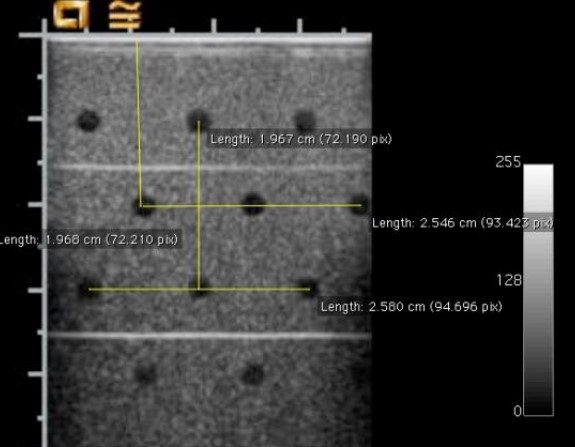
\includegraphics[width=0.6\linewidth]{hv.jpg}
    \caption{\small{Horizontal and vertical Distance Accuracy test}}
    \label{fig:Horizontal and vertical Distance Accuracy}
\end{figure}
\subsubsection{Volume Measurement}
In 3D ultrasound, volumetric information heavily depends on accuracy of the linear measurements in all three dimensions. Therefore it is necessary to evaluate this using the same procedure described above using 3D targets. 


\subsection{Spatial resolution test}
Minimum spatial resolution is the smallest separation that can be seen on the image. Evaluation of spatial resolution might also be performed by using pixel data across a bright target, then plotting to determine FWHM. Both are affected by the gain and gray scale processing settings
Following diagram shows a method of spatial resolution measurement. 

\begin{figure}[h!]
  \centering
  \begin{subfigure}[b]{0.35\linewidth}
    \centering
    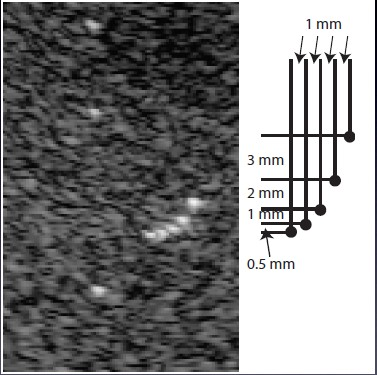
\includegraphics[width=1\linewidth]{q.jpg}
    \caption{Qualitative}
  \end{subfigure}
  \begin{subfigure}[b]{0.6\linewidth}
    \centering
    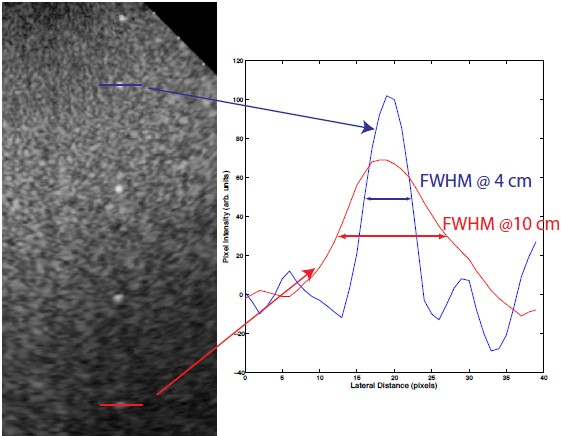
\includegraphics[width=1\linewidth]{sq.jpg}
    \caption{Semi-qualitative}
  \end{subfigure}
  \caption{Spatial resolution test}
  \label{fig:Projectional Radiography}
\end{figure}

Spatial resolution is,
\begin{itemize}
    \item Frequency/transducer dependent
    \item Depth dependent
    \item specified at a frequency and a depth of phantom
\end{itemize}

\subsection{Contrast Resolution test}
\subsubsection{High Contrast Detectability test - Anechoic objects}

Ability to detect anechoic(weakly echogenic objects which reflects sound waves weakly) objects in off-axis is known as contrast resolution. Example for an anechoic object is a cyst. Weakly echogenic objects such as blood vessels also get affected by this. Clutter can be caused by several sources such as S side lobes, quantization clutter and grating lobes. 

Contrast Resolution in this case is defined in terms of Clutter Energy to Total Energy Ratio (CTR). This is measured by taking the average pixel intensity of a cyst phantom image compared to the surrounding.
\begin{figure}[!h]
    \centering
    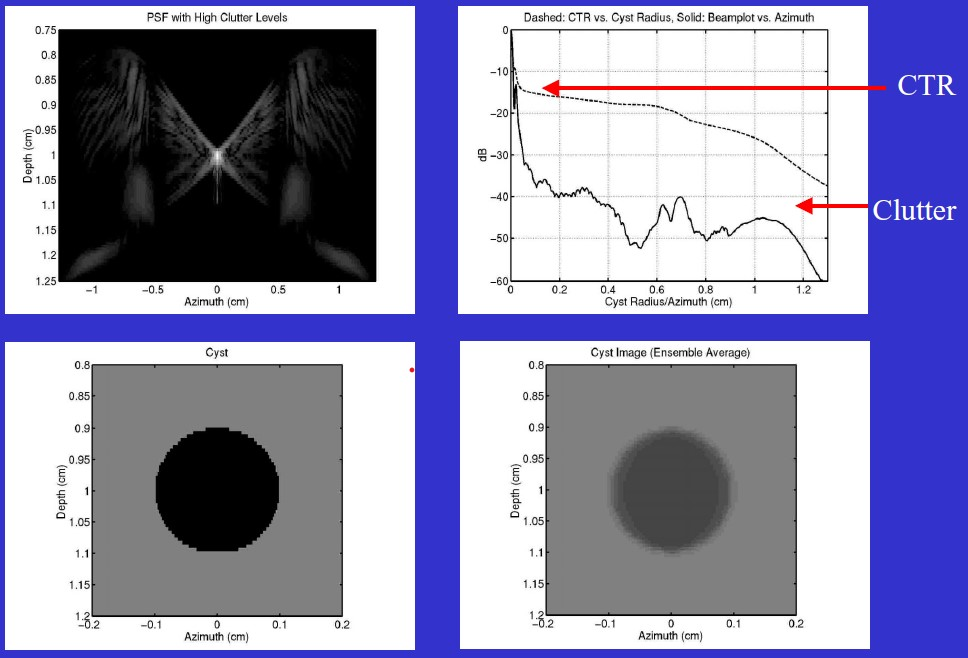
\includegraphics[width=\linewidth]{clutter.jpg}
    \caption{\small{High Contrast Detectability test}}
    \label{fig:High Contrast Detectability test}
\end{figure}

\subsubsection{Low Contrast Object Detectability test - Soft tissue}
Low contrast resolution/ soft tissue resolution refers to the ability to distinguish echogenicity differences between neighboring soft tissue regions. 
As example,
\begin{itemize}
    \item a hyper-echoic or hypo-echoic lesion in normal soft tissue (liver parenchyma)
    \item different types of tissue side by side(liver/bowel/kidney/liver)
\end{itemize}

Speckles in ultrasound images makes detecting subtle echogenicity variations difficult. Tissue contrast resolution can be increased by reducing speckle variance or by reducing speckle size.
\begin{figure}[!h]
    \centering
    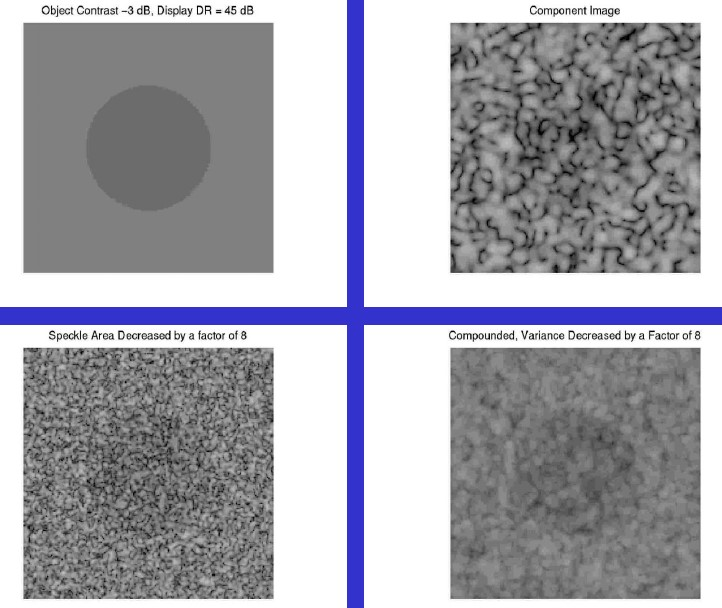
\includegraphics[width=0.8\linewidth]{low.jpg}
    \caption{\small{Low Contrast Detectability test}}
    \label{fig:Low Contrast Detectability test}
\end{figure}

\pagebreak
\section{Recent advancements in \thetitle}
Diagnostic Ultrasound systems are simple when compared with other imaging modalities. They have developed very well and can be assumed as its peak now. However, currently many research efforts are carried out to discover new ways to enhance the level of quality assurance of ultrasound imaging. Some of the quality assurance researches related to Ultrasound imaging quality assurance can be listed as follows. 
\begin{itemize}
    \item Image quality improvements
    \item Advancements in volumetric ultrasound
    \item Ultrasound in every physician’s pocket
    \item Sonoelastography
\end{itemize}


%\pagebreak
\section{Reference}
\begin{enumerate}

    \item Dudley, N., Russell, S., Ward, B., Hoskins, P., \& BMUS QA Working Party. (2014, February). BMUS guidelines for the regular quality assurance testing of ultrasound scanners by sonographers. Retrieved May 17, 2020, from https://www.ncbi.nlm.nih.gov/pmc/articles/PMC4760519/
    \item “Medical ultrasound,” Wikipedia, 17-May-2020. [Online]. Available: https://en.wikipedia.org/wiki/Medical\_ultrasound. [Accessed: 18-May-2020].
    \item A. R. Webb, Introduction to biomedical imaging. Hoboken, N. J.: John Wiley \& Sons, 2006.
    \item Evan J. Boote, Ph.D. University of Missouri-Columbia "Current Ultrasound Quality Control Recommendations and Techniques" 
    \item Kutay F. Üstüner and Gregory L. Holley Siemens Medical Solutions USA, Inc. Ultrasound Division Mountain View, "CA Ultrasound Imaging System Performance Assessment"
    \item “Home,” RSS. [Online]. Available: http://www.aapm.org/. [Accessed: 18-May-2020].
    
    
\end{enumerate}
\pagebreak
\textbf{\Large{Appendix}}
\begin{appendix}
  \listoffigures
  %\listoftables
\end{appendix}

\end{document}

